

\StartOf{Lecture 3}

\Today{Orthogonal Signal Representations: (1) Span, (2) Synthesis, (3) Analysis}

\announcements{
\begin{itemize}
  \item For today:  Rice 5.1; For Mon: Rice 2.5-2.7 and Rice 6.2.1.
  \item HW 1 due a week from today at 11:59pm
  \item Office hours Friday 2:30-3:45pm; please email or use the discussion board for HW questions next week.
  \item I'm out of the country for a conference Mon-Thu next week. Dr.\ Alemayehu Solomon Abrar will be doing a lecture on Mon Jan 27.  There will be no class on Wed Jan 29.
\end{itemize}
}

\section{Orthonormal Signal Representations}

%Last time we defined the term ``orthogonal'' for a pair or set of functions.  I mentioned that a transmitter has a list of possible symbols to send (linear combinations of these waveforms); and that a receiver can estimate the particular amount of each waveform that was sent.  Today we are going to present \emph{how} the transmitter and receiver do both of these things.

We've been talking about orthogonal waveforms. A shorthand notation: the integral of the product of two functions is also called the inner product, and sometimes the notation is used, where $f(t)$ and $g(t)$ are two waveforms:
\[
 \langle f(t), g(t) \rangle = \intinfty{t}{f(t) g(t)}
\]

Recall the definition of an orthonormal basis as given in the previous lecture.

\Definition{Orthonormal}{A set of functions $\phi_0(t), \ldots, \phi_{K-1}(t)$ are \emph{orthonormal} (also referred to as an \emph{orthonormal basis}) if they are mutually orthogonal and each has unit energy, \ie, $\intinfty{t}{ |\phi_k(t)|^2} = 1$ for $k=0,1$.}

Sometimes an orthonormal basis is also called an orthonormal set. There is no difference between the two terms.  The word ``basis'' is nice because it implies you can build something out of the set -- and in fact, you can build a variety of signals by taking some linear combination of the functions in the orthonormal basis.  

For shorthand, we use a set name to describe the orthonormal basis.  The Rice book uses $\mathcal{B}$:
\[
 \mathcal{B} = \{ \phi_0(t), \phi_1(t), \ldots, \phi_{K-1}(t) \}
\]

Each function in $\mathcal{B}$ is called a basis function. You can
think of $\mathcal{B}$ as an unambiguous and useful language.  

What are some common orthonormal bases?
\begin{itemize}
 \item Nyquist sampling: sinc functions centered at sampling times.
 \item Fourier series: complex sinusoids at different frequencies
 \item Sine and cosine at the same frequency
 \item Wavelets
\end{itemize}
And, we will come up with others.  Each one has a limitation -- only a certain set of signals can be exactly represented as a linear combination of its waveforms.  Essentially, we must limit the set of possible signals to a set.  That is, some subset of all possible signals.


\subsection{Span of an Orthonormal Basis}

\Definition{Span}{The span of the set $\mathcal{B}$ is the set of
all functions which are linear combinations of the functions in
$\mathcal{B}$.  The span is referred to as $\Span{B}$ and is
\[
 \Span{B} = \left\{ \sum_{k=0}^{K-1} a_k \phi_k(t)  \mbox{ such that } a_0, \ldots,
 a_{K-1} \in \mathbb{R} \right\}
\]
Another way to define this set is to say that a function $f(t)\in \Span{B}$ if and only if there exists $a_0, \ldots, a_{K-1} \in \mathbb{R}$ such that 
 \[
  f(t) = \sum_{k=0}^{K-1} a_k \phi_k(t)
 \]
}

Recall that we said in Lecture 2 that our modulation scheme is a set of $M$ different linear combinations of $\phi_0(t)$ through $\phi_{K-1}(t)$.  In particular, our transmitter will select symbols of the form
\[
 s_m(t) = a_{m,0} \phi_0(t) + a_{m,1} \phi_1(t) + \cdots + a_{m,K-1} \phi_{K-1}(t) 
\]
for $m=0$ to $M-1$.  Clearly, all symbols $s_m(t) \in \Span{B}$.  We call the set of the $M$ possible symbols $\mathcal{S}$.  That is,
\[
 \mathcal{S} = \{ s_0(t), \ldots, s_{M-1}(t)\}.
\]
Since every element of $ \mathcal{S} \in \Span{B}$, it is clear that $ \mathcal{S} \subset \Span{B}$.


\subsection{Synthesis}

Consider that you have a symbol waveform you want to send, $s_m(t)$, and that you know that it is in the span of your basis $\mathbf{B}$.  Then it can be represented
as a linear combination of the basis functions,
\[
  s_m(t) = \sum_{k=0}^{K-1} a_{m,k} \phi_k(t)
\]
Further, we can calculate the particular constants $a_{m,k}$ using the inner product:
\[
  a_{m,k} = \langle s_m(t), \phi_k(t) \rangle
\]
The \emph{projection} of the $m$th symbol $s_m(t)$ onto basis function $k$ is
defined as $a_{m,k} \phi_k(t) = \langle s_m(t), \phi_k(t) \rangle
\phi_k(t)$. Then the signal is equal to the sum of its projections
onto the basis functions.

\textbf{Why is this?}

\Solution{ Since $s_m(t) \in \Span{B}$, we know there are some
constants $\{a_{m,k}\}_k^{K-1}$ such that
\[
   s_m(t) =  \sum_{k=0}^{K-1} a_{m,k} \phi_k(t)
\]
Taking the inner product of both sides with $\phi_j(t)$,
\begin{eqnarray}
  \langle s_m(t), \phi_j(t) \rangle &=&
     \left\langle \sum_{k=0}^{K-1} a_{m,k} \phi_k(t), \phi_j(t) \right\rangle \nnn
  \langle s_m(t), \phi_j(t) \rangle &=&
     \sum_{k=0}^{K-1} a_{m,k} \langle \phi_k(t), \phi_j(t) \rangle \nnn
  \langle s_m(t), \phi_j(t) \rangle &=&  a_{m,j} \nn
\end{eqnarray}
}

So, now we can now represent a signal by a vector,
\[
  \mbs_i = [ a_{i,0}, a_{i,1}, \ldots, a_{i,K-1}]^T
\]
This and the basis functions \textbf{completely represent each
signal}. Plotting $\{\mbs_i\}_i$ in an $K$ dimensional grid is
termed a \emph{constellation diagram}.  Generally, this space that
we're plotting in is called \emph{signal space}.

We can also synthesize any of our $M$ signals in the signal set by
adding the proper linear combination of the $K$ orthonormal waveforms.  By choosing
one of the $M$ signals, we convey information, specifically, $\log_2
M$ bits of information.  


\begin{figure}[htbp]
  \centerline{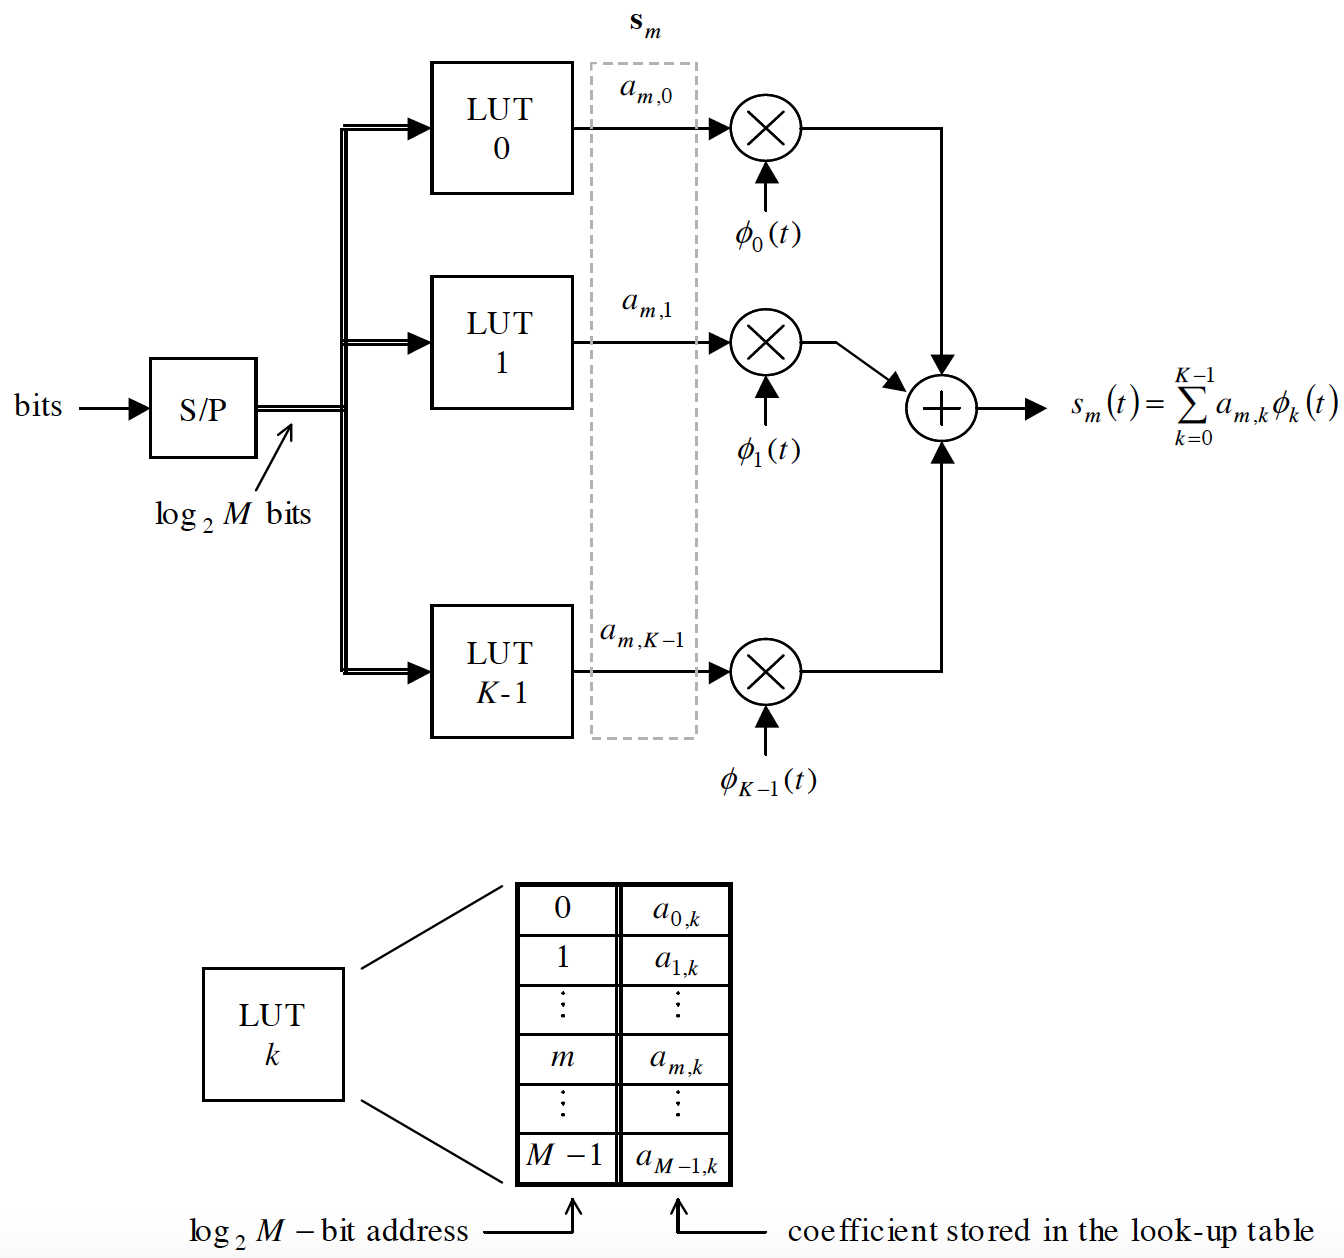
\includegraphics[width=0.8\textwidth]{RiceFigure5-5.png}
  }
  \caption{Rice book Figure 5.5: Block diagram of a modulator for M-ary linear modulation based on the synthesis
equation.}
  \label{F:SynthesisEquationFig}
\end{figure}

See Figure \ref{F:SynthesisEquationFig}, from Rice Chapter 5, which shows a block diagram of how a transmitter would synthesize one of the $M$ signals to send, based on an input bitstream.


\Example{Position-shifted pulses} Plot the signal space diagram for
the signals,
\begin{eqnarray}
  s_0(t) &=& u(t) - u(t-1) \nonumber \\
  s_1(t) &=& u(t-1) - u(t-2) \nonumber \\
  s_2(t) &=& u(t) - u(t-2) \nonumber
\end{eqnarray}
given the orthonormal basis,
\begin{eqnarray}
  \phi_0(t) &=& u(t) - u(t-1) \nonumber \\
  \phi_1(t) &=& u(t-1) - u(t-2) \nonumber
\end{eqnarray}
What are the signal space vectors, $\mbs_0$, $\mbs_1$, and $\mbs_2$?

\Solution{They are $\mbs_0 = [1, 0]^T$, $\mbs_1 = [0, 1]^T$, and
$\mbs_2 = [1, 1]^T$. They are plotted in the signal space diagram in
Figure \ref{F:SampleSpacePosition}.

\begin{figure}[htbp]
  \centerline{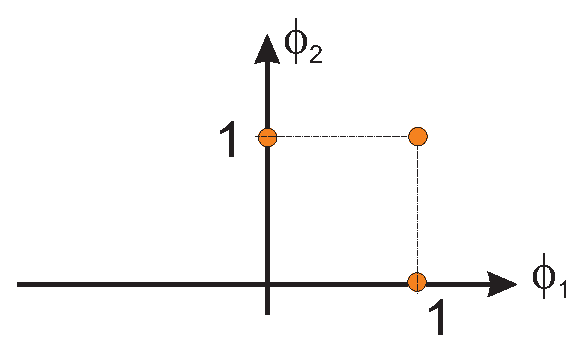
\includegraphics[width=0.4\textwidth]{../images/SignalSpaceExample1.eps}}
  \caption{Signal space diagram for position-shifted signals example.}
  \label{F:SampleSpacePosition}
\end{figure}
}

Energy:
\begin{itemize}
  \item Energy can be calculated in signal space as
    \[
      \mbox{Energy}\{s_m(t)\} = \int_{-\infty}^{\infty}  s_i^2(t) dt = \sum_{k=0}^{K-1}  a_{m,k}^2
    \]
    Proof?
  \item We will find out later that it is the distances between
    the points in signal space which determine the bit error rate
    performance of the receiver.
    \[
      d_{i,j} = \| \mbs_i - \mbs_j \| = \sqrt{\sum_{k=0}^{K-1} (a_{i,k} - a_{j,k})^2 }
    \]
    for $i,j$ in $\{0, \ldots, M-1\}$.  The norm $\| \cdot \|$ given above is the Euclidean norm.
  \item Although different orthonormal bases can be used (one can represent the same symbols with a different orthonormal basis and different symbol vectors), the energy and
    distance between points will not change.
\end{itemize}

\Example{Amplitude-shifted signals} Now consider
\begin{eqnarray}
  s_0(t) &=& 1.5[u(t) - u(t-1)] \nonumber \\
  s_1(t) &=& 0.5[u(t) - u(t-1)] \nonumber \\
  s_2(t) &=& -0.5[u(t) - u(t-1)] \nonumber \\
  s_3(t) &=& -1.5[u(t) - u(t-1)] \nonumber
\end{eqnarray}
and the orthonormal basis,
\begin{eqnarray}
  \phi_1(t) &=& u(t) - u(t-1) \nonumber
\end{eqnarray}
What are the signal space vectors for the signals $\{s_m(t)\}$? What
are their energies?


\Solution{  $\mbs_0 = [1.5]$, $\mbs_1 = [0.5]$, $\mbs_2 = [-0.5]$,
$\mbs_3 = [-1.5]$.  See Figure \ref{F:SampleSpaceAmplitude2}.

\begin{figure}[htbp]
  \centerline{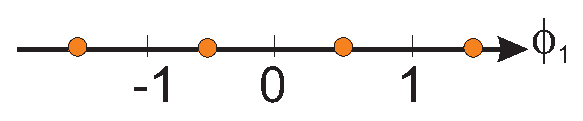
\includegraphics[width=0.4\textwidth]{../images/SignalSpaceExample2.eps}}
  \caption{Signal space diagram for amplitude-shifted signals example.}
  \label{F:SampleSpaceAmplitude2}
\end{figure}

Energies are just the squared magnitude of the vector: 2.25, 0.25,
0.25, and 2.25, respectively. }


\subsection{Analysis}

At a receiver, our job will be to analyze the received signal (a function) and to decide which of the $M$ possible signals was sent. This is the task of \emph{analysis}.  It turns out that an orthonormal bases makes our analysis very straightforward and elegant.

We won't receive exactly what we sent - there will be additional
functions added to the signal function we sent.
\begin{itemize}
  \item Thermal noise
  \item Interference from other users
  \item Self-interference (leftovers from what our transmitter recently sent)
\end{itemize}
We might say that if we send signal $m$, \ie, $s_m(t)$ from our signal set, then we would
receive
\[
  r(t) = s_m(t) + w(t)
\]
where the $w(t)$ is the sum of all of the additive signals that we
did not intend to receive.  But  $w(t)$ would generally not be totally  in the span of our basis $\mathcal{B}$, so $r(t)$ would not be in $\Span{B}$ either.  


\subsubsection{Symbol Closest to Received Signal}

One main question we ask at the receiver is, what is the symbol $s_m(t)$ that is closest to the received signal?  The term ``closest'' here is somewhat qualitative until we define it.  Without proof (in this lecture) we are going to use squared error to measure ``closeness'':
\begin{equation}
 \mathcal{E}_m = \int_{-\infty}^\infty |r(t) - s_m(t)|^2 dt
\end{equation}
That is, for any given $m$, we would integrate across time the squared difference between $r(t)$ and $s_m(t)$.  Our decision will be the $m$ that has minimum $\mathcal{E}_m$:
\begin{equation}
 \hat{m} = \arg \min_{m \in \{0 \ldots M-1\}}  
     \left\{ 
         \int_{-\infty}^\infty |r(t) - s_m(t)|^2 dt
     \right\}
\end{equation}
The term $\hat{s}(t)$ is the result, the receiver's guess of the transmitted symbol.  Because $s_m(t) \in \mathcal{S}$, we know that $s_m(t) = \sum_{k=0}^{K-1} a_{m,k} \phi_{m,k}$.  So,
\begin{eqnarray}
\hat{m} &=& \arg \min_{m \in \{0 \ldots M-1\}} 
     \left\{ 
         \intinfty{t}{ r^2(t)} \right. \nnn
  &&     - 2 \sum_{k=0}^{K-1} a_{m,k} \intinfty{t}{ r(t)\phi_k(t)}  \nnn
  && \left.
         + \sum_{k=0}^{K-1} \sum_{k'=0}^{K-1} a_{m,k} a_{m,k'} \intinfty{t}{ \phi_k(t)\phi_{k'}(t)} 
     \right\}.
\end{eqnarray}
Although there are a lot of terms, this begins to simplify.  The first term is not a function of $m$.  The integral in the second term is the inner product $\langle r(t),\phi_k(t)\rangle$.  Let's call this $x_k$.  The integral in the third term is one when $k=k'$ and zero otherwise, so we can just consider the terms when $k=k'$,
\begin{equation}
 \arg \min_{m \in \{0 \ldots M-1\}} 
     \left\{ - 2 \sum_{k=0}^{K-1} a_{m,k} x_k + \sum_{k=0}^{K-1} a^2_{m,k}
     \right\}.
\end{equation}
We can make this easier for us by including a constant $\sum_{k=0}^{K-1} x^2_k$. Since this constant is not a function of $m$, it doesn't affect the arg min.
\begin{eqnarray}
 &=& \arg \min_{m \in \{0 \ldots M-1\}} 
     \left\{ \sum_{k=0}^{K-1} \left( x^2_k - 2  a_{m,k} x_k + a^2_{m,k} \right)
     \right\}. \nnn
 &=&  \arg \min_{m \in \{0 \ldots M-1\}} 
     \left\{ \sum_{k=0}^{K-1} \left( x_k -  a_{m,k}\right)^2
     \right\}. \nnn
\end{eqnarray}
To find the $m$ that makes this the smallest, then, we should calculate the $x_k$ values by finding the inner product between the received signal and $\phi_k(t)$, and forming the vector
\[
 \mbx = [ x_0, x_1, \ldots, x_{K-1}]^T
\]
Keep a list of the symbol vectors $\mbs_m$ for each $m$.  The final expression above translates to 
\begin{equation}
\hat{m} = \arg \min_{m} \| \mbx - \mbs_m \|^2
\end{equation}
where $\| \cdot \|^2$ is the squared norm of a vector.  Thus, just find the squared Euclidean distance between each $\mbs_m$ and $\mbx$.  This lowest-squared distance vector corresponds to the $m$ that is closest to the received signal.

Note that $\mbx$, that is, the inner products 
\[
 x_k = \intinfty{t}{ r(t)\phi_k(t)}
\]
are all that matters in the decision about which symbol was sent.  



\subsubsection{Best Approximation for Received Signal in the Basis}

What is the best approximation to $r(t)$ in the
signal space?  Specifically, what is $\hat{r}(t) \in \Span{B}$ such
that the energy of the difference between $\hat{r}(t)$ and $r(t)$ is
minimized, \ie,
\begin{equation} \label{E:ProjectionError}
  \arg \min_{\hat{r}(t) \in \Span{B}} \int_{-\infty}^\infty | \hat{r}(t) - r(t) |^2 dt
\end{equation}

\Solution{ Since $\hat{r}(t) \in \Span{B}$, it can be represented as
a vector in signal space,
\[
  \mbx = [x_0, x_1, \ldots, x_{K-1} ]^T.
\]
and the synthesis equation is
\[
  \hat{r}(t) = \sum_{k=0}^{K-1} x_k \phi_k(t)
\]
If you plug in the above expression for $\hat{r}(t)$ into
(\ref{E:ProjectionError}), and then find the minimum with respect to
each $x_k$, you'd see that the minimum error is at
\[
x_k = \int_{-\infty}^\infty r(t) \phi_k(t) dt
\]
that is, $x_k = \langle r(t), \phi_k(t) \rangle$, for $k=0, \ldots,
K-1$. }

\Example{ Analysis using a Walsh-Hadamard 2 Basis}  See Figure
\ref{F:SignalSpaceAnalysisExample}.   Let $s_0(t) = \phi_0(t)$ and 
$s_1(t) = \phi_1(t)$. What is $\hat{r}(t)$?

\begin{figure}[htbp]
  \centerline{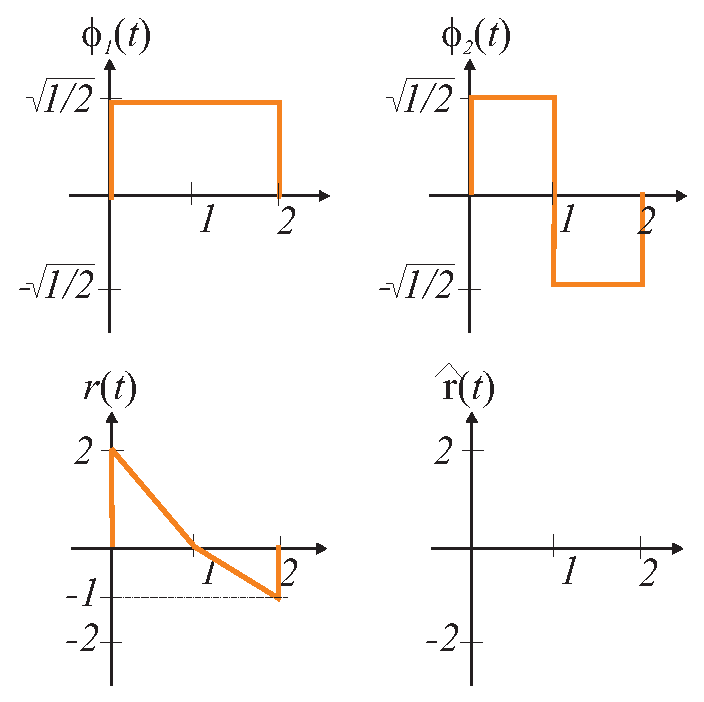
\includegraphics[width=0.6\textwidth]{../images/SigSpace-Analysis-EgProblem.eps}}
  \caption{Signal and basis functions for Analysis example.}
  \label{F:SignalSpaceAnalysisExample}
\end{figure}

\Solution{
\[
 \hat{r}(t) = \pdfarrays{1}{0 \le t < 1}{-1/2}{1 \le t < 2}
\]
}
%\section{Gram-Schmidt Algorithm}
%
%How do you come up with orthonormal bases?  This section presents
%the Gram-Schmidt algorithm.  This material is heavy in calculations,
%easy to make mistakes, and as such not required material for this
%course. But, you should know what it does so that you can use the
%equivalent Matlab script to generate an orthonormal basis.
%
%\begin{figure}[h]
%  \centerline{\psfig{figure=FourPulses-Problem-7-6.eps,width=3in}}
%  \caption{Four signals used to send 2 bits of information.}
%  \label{F:Sampling-FreqDomain}
%\end{figure}
%
%\Example{Taken from Proakis \& Salehi} Consider a transmitter which
%sends one the following transmitted waveforms in order to convey
%data. We might use $s_1(t)$ to transmit a `01', $s_2(t)$ to transmit
%a `10', $s_3(t)$ to transmit a `11', and $s_4(t)$ to transmit a
%`00'.
%\begin{enumerate}
% \item What is an orthonormal basis for these four signals?
%\end{enumerate}
%
%Solution:  Use Gram-Schmidt algorithm.
%
%Round 1:  Select signal $s_1(t)$ and normalize it to find the first
%basis function,
%\[
%  \phi_1(t) = \frac{s_1(t)}{\|s_1(t)\|}
%\]
%Then, start round $k=2$ and repeat the following steps:
%\begin{enumerate}
%  \item \emph{Compute Projections}:  Calculate the inner product of $s_{k}(t)$
%    with the basis functions so far,
%    \begin{eqnarray}
%      c_{k,1} &=& \langle s_{k}(t), \phi_1(t) \rangle \nonumber \\
%        \vdots && \vdots \nonumber \\
%      c_{k,k-1} &=& \langle s_{k}(t), \phi_{k-1}(t) \rangle \nonumber
%    \end{eqnarray}
%  \item \emph{Subtract Projections}: Calculate an
%    orthogonal function $d_k(t)$ as,
%    \begin{equation}
%      d_k(t) = s_k(t) - \sum_{i=1}^{k-1} c_{k,i} \phi_i(t)
%    \end{equation}
%  \item \emph{Check for Stopping Condition}:  If $d_k(t) = 0$ for all $t$,
%    then no new basis function is created.  If $d_k(t) \neq 0$ then
%    do the next step.
%  \item \emph{Normalize}:  Create a new basis function,
%    \[
%      \phi_k(t) = \frac{d_k(t)}{\|d_k(t)\|}
%    \]
%    Repeat 1-4 until $k=M$.
%\end{enumerate}
%The value $N$ is the number of new basis functions created.  This is
%the minimum $N$ functions which can form an orthogonal basis for
%$\{s_m(t)\}$.
%
%\Note{You can order the signals $s_m(t)$ in any order.  You may get
%different bases, but $N$ will be the same.}
%
%
%\Example{Example from Proakis \& Salehi} Starting with $s_1(t)$,
%first calculate $\phi_1(t)$:
%\[
%  \phi_1(t) = \frac{2[u(t) - u(t-3)]}{\sqrt{4\cdot 3}}
%            = \frac{u(t) - u(t-3)}{\sqrt{3}}
%\]
%Start the 4-step process.  For $k=2$,
%\begin{enumerate}
%  \item \emph{Compute Projections}:
%    \begin{eqnarray}
%      c_{2,1} &=& \langle s_{2}(t), \phi_1(t) \rangle =  \int_0^1 \frac{2}{\sqrt{3}} dt = \frac{2}{\sqrt{3}}  \nonumber
%    \end{eqnarray}
%  \item \emph{Subtract Projections}:
%    \begin{eqnarray}
%      d_2(t) &=& s_2(t) - c_{2,1}\phi_1(t)
%        \nonumber \\
%      d_2(t) &=& 2[u(t) - u(t-1)] - \frac{2}{\sqrt{3}}\frac{u(t) - u(t-3)}{\sqrt{3}}
%        \nonumber \\
%      d_2(t) &=& 2[u(t) - u(t-1)] - \frac{2}{3}[u(t) - u(t-3)]
%        \nonumber \\
%      d_2(t) &=& \frac{4}{3}[u(t) - u(t-1)] + \frac{-2}{3}[u(t-1) - u(t-3)]
%        \nonumber
%    \end{eqnarray}
%  \item \emph{Check for Stopping Condition}:  $d_k(t) \neq 0$.
%  \item \emph{Normalize}:
%    \begin{eqnarray}
%      \|d_2(t)\|^2 &=& \int_0^1 \frac{16}{9} + \int_1^3 \frac{4}{9} = \frac{16 +
%        8}{9} = \frac{8}{3} \nonumber \\
%      \phi_2(t) &=& \sqrt{\frac{3}{8}} d_k(t)
%                = \sqrt{\frac{2}{3}}[u(t) - u(t-1)]
%                  + \frac{-1}{\sqrt{6}}[u(t-1) - u(t-3)]
%                \nonumber
%    \end{eqnarray}
%\end{enumerate}
%For $k=3$,
%\begin{enumerate}
%  \item \emph{Compute Projections}:
%    \begin{eqnarray}
%      c_{3,1} &=& \langle s_{3}(t), \phi_1(t) \rangle
%               = \int_1^3 -2\frac{1}{\sqrt{3}} dt = \frac{-4}{\sqrt{3}}
%               \nonumber \\
%      c_{3,2} &=& \langle s_{3}(t), \phi_2(t) \rangle
%               = \int_1^3 -2 \frac{-1}{\sqrt{6}} dt = \frac{4}{\sqrt{6}}  \nonumber
%    \end{eqnarray}
%  \item \emph{Subtract Projections}:
%    \begin{eqnarray}
%      d_3(t) &=& s_3(t) - c_{3,1}\phi_1(t) - c_{3,2}\phi_2(t)
%        \nonumber \\
%      d_3(t) &=& -2[u(t-1) - u(t-3)] \nonumber \\ &&+ \frac{4}{\sqrt{3}}\frac{u(t) - u(t-3)}{\sqrt{3}}
%              \nonumber \\ &&     - \frac{4}{\sqrt{6}} \left\{
%                       \sqrt{\frac{2}{3}}[u(t) - u(t-1)] + \frac{-1}{\sqrt{6}}[u(t-1) - u(t-3)]
%                     \right\}
%        \nonumber \\
%      d_3(t) &=& -2[u(t-1) - u(t-3)] \nonumber \\
%             &&    + \frac{4}{3}[u(t) - u(t-3)]\nonumber \\
%             &&    - \frac{4}{3}[u(t) - u(t-1)] + \frac{2}{3}[u(t-1) - u(t-3)] \nonumber \\
%             &=& 0
%        \nonumber
%    \end{eqnarray}
%  \item \emph{Check for Stopping Condition}:  $d_k(t) = 0$:  no new
%  basis function.
%\end{enumerate}
%For $k=4$,
%\begin{enumerate}
%  \item \emph{Compute Projections}:
%    \begin{eqnarray}
%      c_{4,1} &=& \langle s_{4}(t), \phi_1(t) \rangle
%               = \int_0^2 2 \frac{1}{\sqrt{3}} dt = \frac{4}{\sqrt{3}}
%               \nonumber \\
%      c_{4,2} &=& \langle s_{4}(t), \phi_2(t) \rangle
%               = 2 \int_0^2 \sqrt{\frac{2}{3}}[u(t) - u(t-1)] + \frac{-1}{\sqrt{6}}[u(t-1) - u(t-3)]  dt
%               \nonumber \\
%               &=& 2 \left( \frac{\sqrt{6}}{3} -\frac{\sqrt{6}}{6} \right) = \frac{\sqrt{6}}{3} \nonumber
%    \end{eqnarray}
%  \item \emph{Subtract Projections}:
%    \begin{eqnarray}
%      d_4(t) &=& s_4(t) - c_{4,1}\phi_1(t) - c_{4,2}\phi_2(t)
%        \nonumber \\
%      d_4(t) &=& 2[u(t) - u(t-2)] - \frac{4}{\sqrt{3}}\frac{u(t) - u(t-3)}{\sqrt{3}}
%       \nonumber \\ &&
%                   - \frac{\sqrt{6}}{3} \left\{
%                       \frac{\sqrt{6}}{3}[u(t) - u(t-1)] - \frac{\sqrt{6}}{6}[u(t-1) - u(t-3)]
%                     \right\}
%        \nonumber \\
%      d_4(t) &=& 2[u(t) - u(t-2)] - \frac{4}{3}[u(t) - u(t-3)]
%       \nonumber \\ &&
%                   - \frac{2}{3} [u(t) - u(t-1)] + \frac{1}{3}[u(t-1) - u(t-3)]
%        \nonumber \\
%      d_4(t) &=&  [u(t-1) - u(t-2)] - [u(t-2) - u(t-3)]
%        \nonumber
%    \end{eqnarray}
%  \item \emph{Check for Stopping Condition}:  $d_k(t) \neq 0$.
%  \item \emph{Normalize}:
%    \begin{eqnarray}
%      \|d_4(t)\|^2 &=& 1+1 = 2 \nonumber \\
%      \phi_4(t) &=& \frac{d_k(t)}{\sqrt{2}}  \nonumber \\
%                &=& \frac{1}{\sqrt{2}}[u(t-1) - u(t-2)] - \frac{1}{\sqrt{2}}[u(t-2) - u(t-3)]
%                \nonumber
%    \end{eqnarray}
%\end{enumerate}
%The basis functions are plotted in Figure \ref{F:GramSchmidt_1}.
%
%\begin{figure}[h]
%  \centerline{\psfig{figure=plotBasisGramSchmidt_1.eps,width=3.5in}}
%  \caption{Three basis functions for Problem 7.6, computed using the signals 1 through 4 in order in the Gram-Schmidt algorithm.}
%  \label{F:GramSchmidt_1}
%\end{figure}
